\subsection{Постановка задачи на разработку программы}
    Цель работы - реализовать программатор для микроконтроллеров PIC серии 16F на тонком клиенте Orange PI Lite.

\bigskip
Задачи работы:

\smallskip
\begin{my_enumerate}
\item Чтение данных из формата INTEL HEX8M для хранения программы прошивки.
\item Возможность отдельной записи EEPROM памяти, не стирая програмную память микроконтроллера.
\item Поддержка 3 линеек микроконтроллеров серии 16F: 627A / 628A / 648A.
\item Проверка входного файла на корректность.
\item Графический интерфейс для оперирования программой.
\item Интерфейс командной строки для оперирования программой.
\item Повышаюший переходник с 3.3В на 5В для взаимодействия с микроконтроллером.
\item Схемотехника для платы которая позволяет подключить микроконтроллер к тонкому клиенту Orange Pi Lite.
\item Завершенные, работающие схемы на макетной плате.
\item Схемы разводки макетной платы для подключения микроконтроллера к Orange Pi Lite. 
\end{my_enumerate}


\subsection{Описание алгоритма и функционирования программы}


%=============================================================
\subsubsection{Выбор алгоритма}

\textbf{Различные подходы}
для программирования (или прошивки) микроконтроллеров варьируются в зависимости от кампании производиля. 
Данная курсовой работы нацелена на создание программатора для определенной серии и линейки микроконтроллеров определенного производителя. Микроконтроллер - микросхема, предназначенная для управления электронными устройствами. Микроконтроллер сочетает на одном кристалле функции микропроцессора, а также и функции периферийных устройств, содержит ОЗУ и ПЗУ. Это однокристальный компьютер, способный выполнять относительно простые задачи.
Имеет смысл упомянуть две большие компании производящие микроконтроллеры общего назначения. А иммено кампанию Microchip, производящую микроконтроллеры PIC и компанию Atmel чьи микроконтроллеры ATmega легли в основу Arduino.

\textbf{Программирование}
PIC16F627A/628A/648A производится с помощью
серийного (последовательного) метода. Серийный режим позволяет
PIC16F627A/628A/648A быть запрограммированым с изпользованием лишь 5 ножек микроконтроллера (или 6 ножек при режиме низковольтного программирования) уже будучи встроенным
в систему пользователя. Это предоставляет большую гибкость в процессе программирования 
(позволяет пользователю более свободно выбирать "место" и "время" для программирования).

\textbf{Вольтаж режима программирования}
определяет если будет использован низковольтный или высоковольтный режим. Использование низковольтного режима позволяет программировать PIC имея в доступноси только источники питания от 2.0В до 5.0В, но требует дополнительной ножки микроконтроллера. Использование только высоковольтных режимов позволяет переопределить ножку PGM микроконтроллера под пользовательские нужды, но требует наличия источника питания на 12В. В данной работе используется низковолтный режим поскольку тонкий клиент Orange Pi Lite не имеет возможности предоставить 12В питание.

\textbf{Режим программирования}
Режим программирования для PIC16F627A/628A/648A позволяет программировать ячейки
 программной памяти, ячейки памяти данных, конфигурациионное слово, а также специальные 7 ячеек, которые используются для храненния ID устройства.

\textbf{Команды программирования} 
в режиме программирования, обмен информацией с PIC определяеться набором команд и  их операндами которые передаются в микроконтроллер и/или обратно через серийные кабели.



%=============================================================
\subsubsection{Основные определения и структуры данных}

\textbf{Ячейки памяти}
в данных микроконтроллерах могут быть как и 14, так и 8 битными. 
На PIC16F627A/628A/648A реализованна Гарвардская
архитектура с отдельными шинами для инструкций и данных, что позволяет 
14-разрядным инструкциям работать с 8-разрядными данными.

\textbf{Пользовательская программа} на тонком клиенте Orange Pi Lite, 
храниться в массиве размером с программируемую память микроконтроллера 
(0х2007 байт) элементов типа unsigned uint_16, из которых для 
данных и для команд используются только нижние 8 и 14 байт 
соответственно. В массиве эта информация хранится непосредственно 
перед побитовой передачей на микроконтроллер.

\textbf{Пространство програмной памяти}
отведенное пользователю простирается от 0x0000 до
0x1FFF. В режиме программирования, пространство программной памяти
простирается от 0x0000 до 0x3FFF, с первой
половиной (от 0x0000-0x1FFF), которая отведена программной памяти, и
второй половиной (0x2000-0x3FFF), которая отведена конфигурационной
памяти. Все другие адреса в конфигурационной памяти PIC зарезервированы 
и не могут быть запрограммированы пользователем.

\begin{figure}[h!]
    \centering
    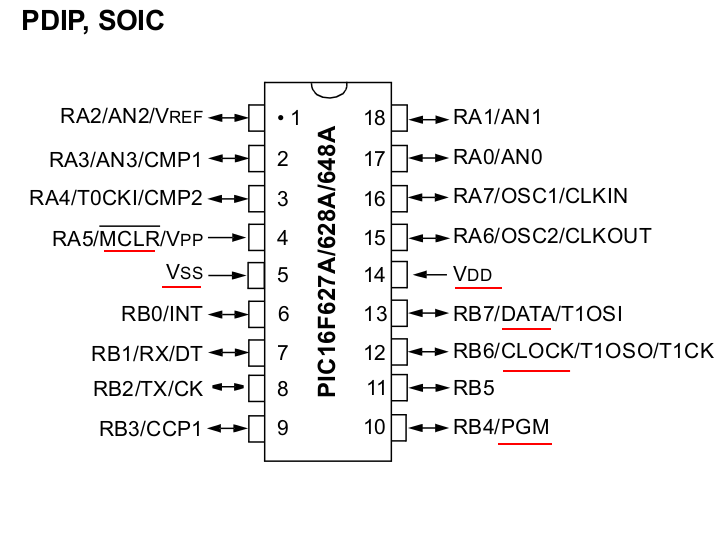
\includegraphics[width=0.8\textwidth]{2017-05-07_at_22:31:52_screenshot.png}
    \caption{Карта памяти микроконтроллера. Белым выделены области для пользовательского кода.}
\end{figure}

\textbf{В пространство конфигурационной памяти}
(адреса 0х2000 - 0х2007) можно войти через послание специальной команды 
"Загрузить даннные для конфигурационной памяти". Только адреса 0x2000-0x200F 
конфигурационного пространства памяти физически реализованы. Однако, только 
ячейки 0x2000 вплоть до 0x2007 доступны для программирования. Остальные ячейки
зарезервированны. Переход по адресу за пределами 0x200F будет физически осуществлять
доступ к пользовательской памяти.

\textbf{Пространство ПЗУ памяти}
простирается от 0x00 до 0xFF и находится отдельно от пространства программной памяти
и пространства оперативной памяти. Для ПЗУ реализуются только нижние 128 байт
для устройств PIC16F627A/628A, в то время как для PIC16F648A
реализуются все 256 байт. Программирование ПЗУ памяти данных использует тот же программный счетчик
что и для программирования конфигурационной и програмной памяти, однако только нижние биты
декодируется и используется. Поэтому перед программированием ПЗУ необходимо чтобы 
программный счетчик указывал на 0х0000 или 0х2000.

\textbf{Создание структуры} для представления памяти микроконтроллера. 
Ключевым элементом в представлении памяти микроконтроллера является массив типа uint16_t размером с память PIC.
Для того чтобы ускорить процесс прошивки микроконтроллера вводятся переменные program_memory_used_cells, и program_memory_max_used_address. Они обозначают общее колличество задействованных программой ячеек памяти, и самый высокий адрес в програмной памяти. Таким образом можно заметить условия при которых можно досрочно закончить программирование програмной памяти PIC и перейти к следующей стадии программирования.

\begin{small}
\begin{verbatim}
struct picmemory {
    uint16_t  program_memory_used_cells;
    uint16_t  program_memory_max_used_address;

    uint8_t   has_configuration_data;
    uint8_t   has_eeprom_data;

    uint16_t *data;     /* 14-bit data */
    uint8_t  *filled;   /* 1 if this cell is used */
};
\end{verbatim}
\end{small}

\textbf{Внутренний програмный}
счетчик может увеличиваться от 0х0000 до 
конца реализованной програмной памяти 0х03FF (или 0x07FF, или 0x0FFF в зависимости от модели PIC)
после чего он вновь обернется на адресс 0х0000.
Для включения высоких бит програмного счетчика и перехода
к программированию конфигурационной памяти, необходимо послать спецальную команду.
Послее нее програмный счетчик будет оперировать в пространстве от 0х2000 до 0х3FFF
(по достижении 0х3FFF он будет вновь оборачиваться на 0х2000). Единственным 
способом сбросить верхние биты програмного счетчика вновь на 0х0000 это покинуть и
повторно войти в режим программирования.

\textbf{Ячейки для ID}
пользователя отображаются на адреса [0x2000 : 0x2003] и являются 
частью конфигурционной памяти. Пользователь может хранить 
идентификационные данные (идентификатор пользователя) в
четырех локациях для идентификатора пользователя. Этот идентификатор всегда можно считать
корректно, даже если будет включена защита кода.

\textbf{Питание}
в режиме программирования. Для PIC16F627A/628A/648A требуется один источник питания с VDD 
(2.0V до 5.5V) и VPP от 12В до 14В, или же VPP от 4.5В до 5.5В, 
при использовании низковольтного программирования. 
Оба источника должны иметь разрешение как минимум в 0,25В.

\textbf{I/O Выходы} используемые для программирования. Положительный входной сигнал на ножке RB4 называемой PGM вводить микроконтроллер в режим низковольтного программирования (если данная опция была включена в конфигурационном слове микроконтроллера). Ножка RB7 называемая DATA, настраивается как вход и используется для по-битовой передачи данных программых в микроконтроллер. Ножка RB6 называемая CLOCK, также настраивается на прием входного сигнала и используется для синхронизации состояния напряжения на ножке RB7. Во время падения напряжения на ножке RB6, микроконтроллер считает следующий бит с ножки RB7. Ножка MCLR/Vpp изпользуется для выбора режима программирования. В PIC16F627A/628A/648A, высокое напряжение для работы с ячейками памяти генерируется автоматически. Для активации
режима программирования, необходимо применить высокое напряжение ко входу MCLR. Поскольку MCLR используется на уровне источника, это означает, что MCLR не тянет какиой-либо значительный ток. Ножка VDD предоставляет 5В необходимые для стабильной работы микроконтроллера в штатном режиме. Ножка VSS определяет напряжение на уровне земли.

\begin{figure}[h!]
    \centering
    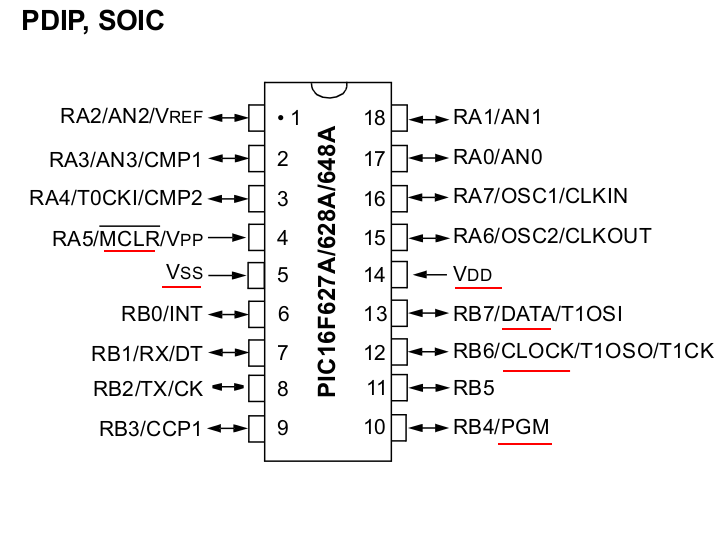
\includegraphics[width=0.8\textwidth]{2017-05-07_at_22:31:52_screenshot.png}
    \caption{I/O выходы необходимые для программирования в серийном режиме}
\end{figure}

\textbf{Команды программирования} 
в режиме программирования, обмен информацией с PIC определяеться набором команд и 
их операндами которые передаются в микроконтроллер и/или обратно через серийные кабели. 
Общая форма для всех последовательностей команд
состоит из 6-битовой команды и условно 16-битного
слова данных. И команды и слова данных передаются начиная с наименее значимого бита (LSB first).
Для других серий и линеек типа PIC набор команд может отличаться.

\begin{figure}[h!]
    \centering
    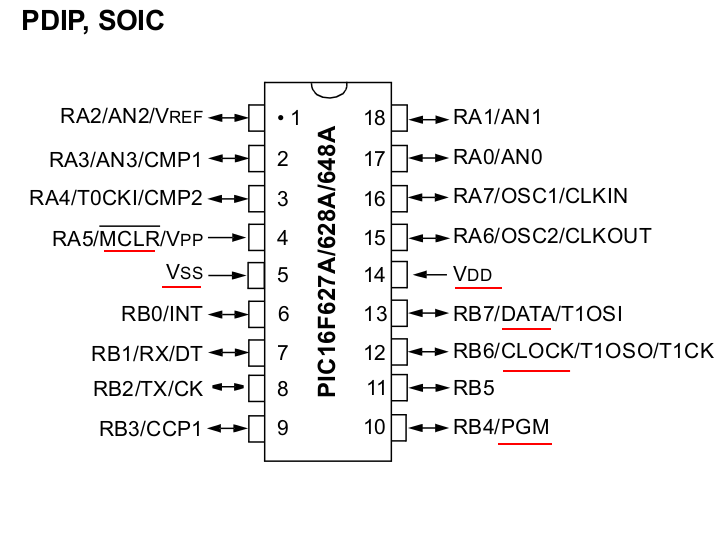
\includegraphics[width=0.8\textwidth]{2017-05-07_at_22:31:52_screenshot.png}
    \caption{Последовательности 6-разрядных команд для PIC16F627A/628A/648A}
\end{figure}

\textbf{Абстрагирование программатора} от конкретной модели микроконтроллера семейства PIC 
делается с помощю определения дополнительной структуры в которой для каждой конкретной модели 
хранится информация о карте памяти, о командах программирования, о задержках необходимых между 
сигнальными последовательностями.

\begin{small}
\begin{verbatim}
struct picmicro {
    uint16_t device_id;
    char     name[16];
    size_t   program_memory_size;
    size_t   data_memory_size;

    int program_cycle_time;     /* in microseconds */   // T_PROG
    int eeprom_program_cycle_time;  // T_DPROG
    int bulk_erase_cycle_time;      // T_ERA

    uint8_t load_configuration_cmd;
    uint8_t load_data_for_program_memory_cmd;
    uint8_t load_data_for_data_memory_cmd;
    uint8_t read_data_from_program_memory_cmd;
    uint8_t read_data_from_data_memory_cmd;
    uint8_t increment_address_cmd;
    uint8_t begin_erase_programming_cycle_cmd;
    uint8_t begin_programming_only_cycle_cmd;
    uint8_t bulk_erase_program_memory_cmd;
    uint8_t bulk_erase_data_memory_cmd;
};
\end{verbatim}
\end{small}

Для микроконтроллеров PIC16F627A/628A/648A используется нижеследующее определение экземпляра данной структуры.
\begin{small}
\begin{verbatim}
const struct picmicro pic16f628a = {
    /* General */
    .device_id =                          0x1060,
    .name =                               "pic16f628a",
    .program_memory_size =                0x800,
    .data_memory_size =                   128,
    
    /* Time intervals in microseconds */
    .program_cycle_time =                 4000,
    .eeprom_program_cycle_time =          6000,
    .bulk_erase_cycle_time =              6000,
    
    /* Commands */
    .load_configuration_cmd =             0x00,
    .load_data_for_program_memory_cmd =   0x02,
    .load_data_for_data_memory_cmd =      0x03,
    .read_data_from_program_memory_cmd =  0x04,
    .read_data_from_data_memory_cmd =     0x05,
    .increment_address_cmd =              0x06,
    .begin_erase_programming_cycle_cmd =  0xFF,
    .begin_programming_only_cycle_cmd =   0x08,
    .bulk_erase_program_memory_cmd =      0x09,
    .bulk_erase_data_memory_cmd =         0x0B
};
\end{verbatim}
\end{small}


%=============================================================
\subsubsection{Описание алгоритма}

\textbf{Чтение файла} с программой пользователя, это первый шаг программатора. Следующим шагом 
являеться проверка входного файла на корректность. Для этого используются особенности формата INTEL HEX8M.

% рассказать про формат привести пример файла в из книги MPASM USER GUIDE

\begin{figure}[h!]
    \centering
    \includegraphics[width=0.8\textwidth]{intel_hex_file_colored_example.png}
    \caption{Пример входного файла к программатору}
\end{figure}


По мере чтения входного файла, по адресу в файле в соответствующий адрес в массиве структуры "picmemory" вставляются значения. 
Поскольку на тонком клиенте Orange Pi Lite установлен little-endian процессор 
компании Allwinner модели H3, а в формате INTEL HEX8M данные записываются в порядке 
MSB, то при вставке в массив необходимо поменять местами верхний и нижний байты.

В цикле происходит прочтение входного файла и создание структуры для представления памяти микроконтроллера.
\begin{small}
\begin{verbatim}
for (i = 0; i < byte_count / 2; i++) {
        nread = sscanf(&line[9+4*i], "%4hx", &data);
	uint16_t pic_data = swap_uint16(data);
        if (nread != 1) {
                fprintf(stderr, "Error: cannot read data.\n");
                free_picmemory(&pm);
                return NULL;
        }
        if (debug)
                fprintf(stderr, "  data        = 0x%04X (file) = 0x%04X (micro)\n", data, pic_data);
        checksum_calculated += (data >> 8) & 0xFF;
        checksum_calculated += data & 0xFF;

        if (address + i < 0x2000) {
                pm->program_memory_used_cells       += 1;
                pm->program_memory_max_used_address  = address + i;
        } else if (0x2000 <= address + i && address + i < 0x2008)
                pm->has_configuration_data = 1;
        else if (address + i >= 0x2100)
                pm->has_eeprom_data = 1;

        pm->data[address + i]   = pic_data;
        pm->filled[address + i] = 1;
}
\end{verbatim}
\end{small}

Программатор работает через посылание 
последовательности команд и данных, введенных в серийном режиме
в котором бит на линии данных загоняется в микроконтроллер на падающем
фронте напряжения на линии часов. Команда + данные, вводятся последовательно, 
через линию часы и линию данных, которые с аппаратной точки зрения являются входными линиями 
изпользующими триггеры Шмитта для различения напряжения 0 или 1. 

\begin{figure}[h!]
    \centering
    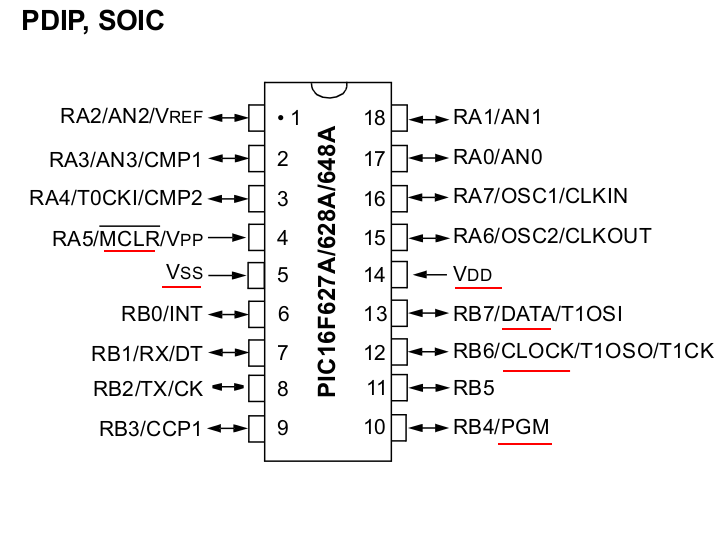
\includegraphics[width=0.8\textwidth]{2017-05-07_at_22:31:52_screenshot.png}
    \caption{Временные интервалы для побитовой передачи команды "Загрузка данных в програмную память"}
\end{figure}


Сигнал на ножке данных имеет минимальные время установки и удержания 
(описанные в таблице ниже, вместе с ограничением по напряжению) по
отношению к падающему фронту напражения на линии часов. Командам, которые
требуют передачи данных, связанных с ними (чтение и запись),
требуется минимальная задержка между передачей команды и передачей данных.

\begin{figure}[h!]
    \centering
    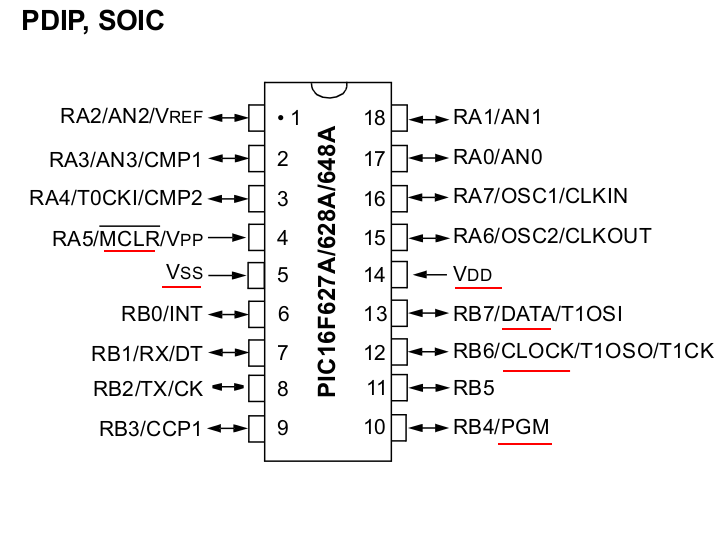
\includegraphics[width=0.8\textwidth]{2017-05-07_at_22:31:52_screenshot.png}
    \caption{Спецификация AC/DC для поднятия/опускания и удержания линий данных и часов}
\end{figure}


\textbf{Точный} алгоритм записи данных в память программы приведен в нижеследующем графе.

\begin{figure}[h!]
    \centering
    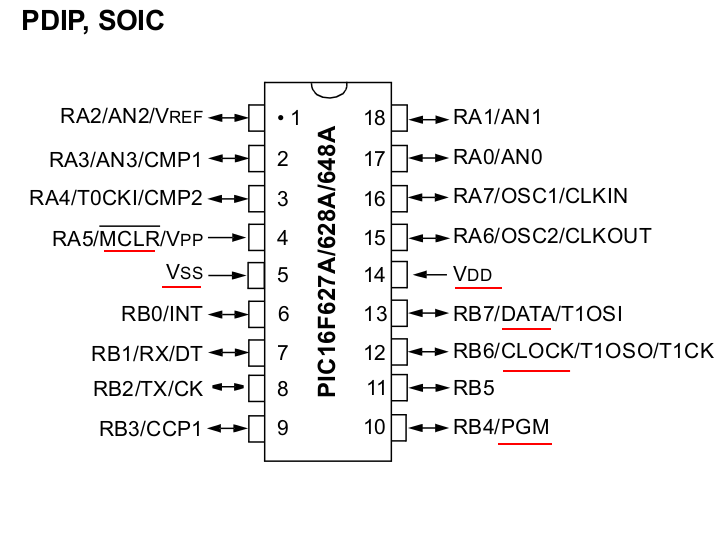
\includegraphics[width=0.8\textwidth]{2017-05-07_at_22:31:52_screenshot.png}
    \caption{Граф алгоритма записи данных в програмную память микроконтроллера}
\end{figure}

\textbf{После создания} карты памяти которая должна быть загруженна в микроконтроллер, следующим 
шагом является непосредственная передача этих данных в PIC. Для этого необходимо получить доступ 
к GPIO выходам тонкого клиента Orange Pi Lite. Со стороны Orange Pi Lite надо было посмотреть на 
поставляемую с ним схемотехнику платы чтобы определить какие выходы PGIO наиболее подходят для работы программатора.
Сигналы передаваемые на ножки микроконтроллера имеют строгие временные рамки, и для того что бы в них вписаться необходимо 
использовать механизм "memory mapped file" для включения и отключения сигналов нв выходах GPIO на уровне процессора.


\begin{figure}[h!]
    \centering
    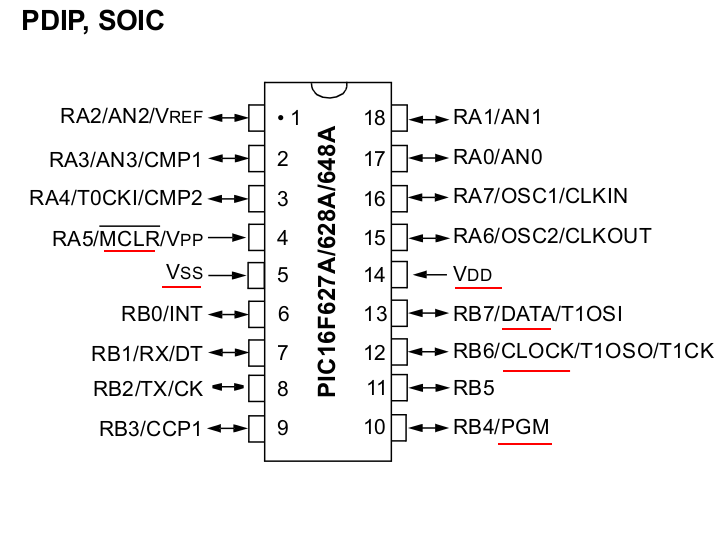
\includegraphics[width=0.8\textwidth]{2017-05-07_at_22:31:52_screenshot.png}
    \caption{Разъем GPIO выходов модели Rasberry Pi B+ которая таже используется и на Orange Pi Lite}
\end{figure}

Посмотрев на схемотехнику для выходов GPIO, решено было выбрать 5 последовательных 
выходов 31, 33, 35, 37, 39 которые подсоедены к процессору Н3 соответственно на ножках 7, 8, 9, 10, 20 порта А.

\begin{figure}[h!]
    \centering
    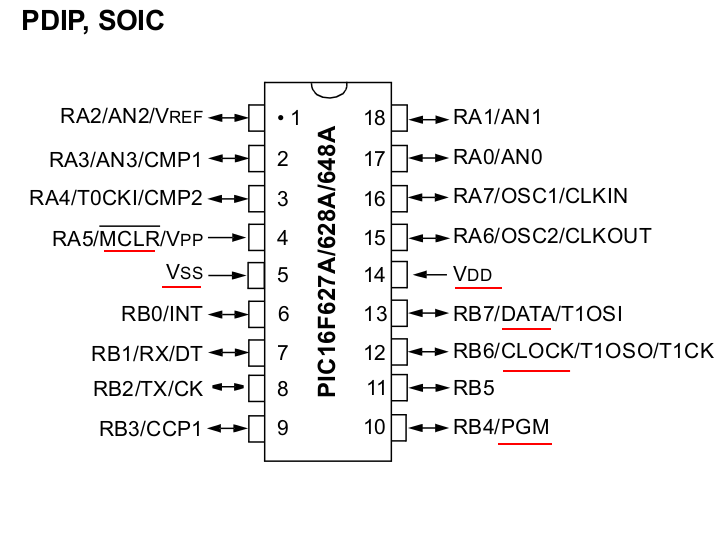
\includegraphics[width=0.8\textwidth]{2017-05-07_at_22:31:52_screenshot.png}
    \caption{Схемотехника для выходов GPIO Orange Pi Lite с процессором H3}
\end{figure}

\begin{figure}[h!]
    \centering
    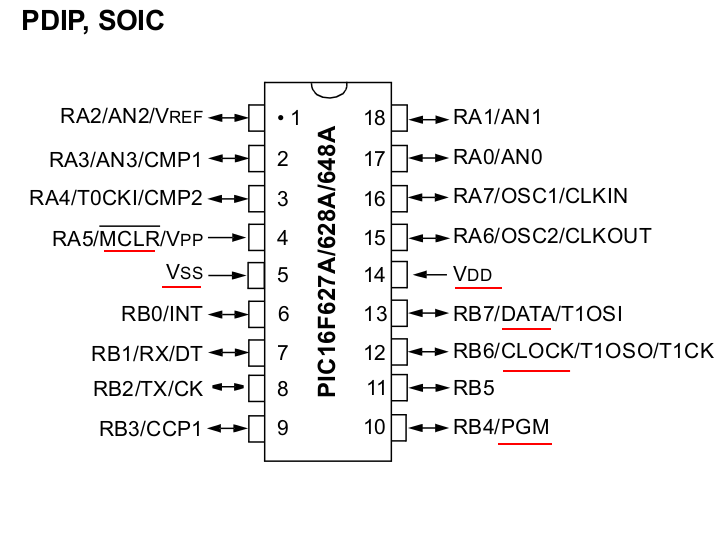
\includegraphics[width=0.8\textwidth]{2017-05-07_at_22:31:52_screenshot.png}
    \caption{Схемотехника для процессора Н3 Orange Pi Lite}
\end{figure}

\textbf{Получение доступа} к выходам GPIO, осуществляется через манипуляцию регистрами отвечающими за порт А напрямую. Для этого делаеться маппинг регистров настройки и состояния порта А в адресоное пространство программы. Значения для адресов регистров и их размера беруться из руководства инженера к процессору Н3.


\begin{figure}[h!]
    \centering
    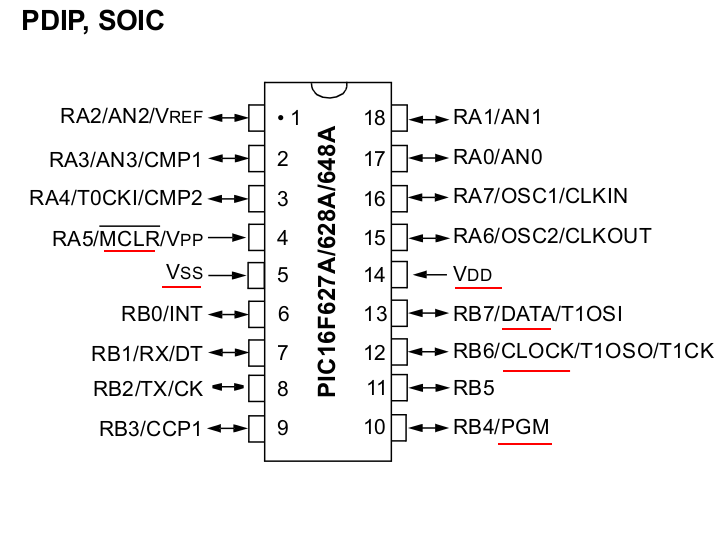
\includegraphics[width=0.8\textwidth]{2017-05-07_at_22:31:52_screenshot.png}
    \caption{Выдержка из руководства инженера к процессору Н3 с адресами ключевых регистров}
\end{figure}

В итоге удалось найти адреса всех регистров влияющих на состояние порта А. Далее приведена краткая сводка констант в которые были записаны необходимые адреса.

\begin{small}
\begin{verbatim}
// AllWinner H3 datasheet, page 86, page 316
uint32_t CCU_BASE = 0x01C20000ul;       // Port controller
uint32_t PIO_OFS =  0x00000800ul;       // GPIO offset

// AllWinner H3 datasheet, page 86, block size is 1024 = 1K = 0x400 bytes 
uint32_t PIO_MAP_LEN = 0x2000;          // Port controller end (0x01C20BFF) - Port controller start (0x01C20800)

// AllWinner H3 datasheet, page 316
uint32_t PA_CFG0_OFS = 0x00000000ul;    //  Port A Configure Register 0
uint32_t PA_CFG1_OFS = 0x00000004ul;    //  Port A Configure Register 1
uint32_t PA_CFG2_OFS = 0x00000008ul;    //  Port A Configure Register 2
uint32_t PA_DAT_OFS  = 0x00000010ul;    //  Port A Data Register
\end{verbatim}
\end{small}


Следом были написанны функции для манипулирования этими регистрами. Ниже приведены фрагменты функций которые ипользуются чтобы выставить состояние ножки GPIO на выход (output) и чтобы менять напряжение на дфнной ножке с 0В до 3.3В. Для регистров бит 0 - это наименее значимый бит.


Ниже приведены фрагменты функций которые ипользуются чтобы выставить состояние ножки GPIO на выход (output) и чтобы менять напряжение на дфнной ножке с 0В до 3.3В. Для регистров бит 0 - это наименее значимый бит.

\begin{small}
\begin{verbatim}


// получение указателя на адрес по которому хранится регистр 
volatile uint32_t* get_data_reg(int pin)
{
    volatile uint32_t* data_reg = (volatile uint32_t * )(gpio + PA_DAT_OFS);
    return data_reg;
}

// создает новое измененное значение для записи в регистр
uint32_t modify_data(uint32_t data, int pin, int value)
{
    uint32_t new_data;
    if (value) {
        new_data = data | (1U << pin);
    }
    else {
        new_data = data & ~(1U << pin);
    }
    return new_data;
}

// выставляет на ножке номер "pin" значение напряжения 0 или 1.
void gpio_wr(int pin, int value) {
    volatile uint32_t* data_reg = get_data_reg(pin);
    uint32_t data = *data_reg;
    uint32_t new_data = modify_data(data, pin, value);
    *(data_reg) = new_data;
}

// модифицирует копию текущих настроек чтобы ножка номер "pin" оказалась настроена как ВЫХОД
// возвращает новое значение которое должно быть записано в регистр
uint32_t modify_cfg_output(uint32_t cfg, int pin)
{
    /* Write value 001 to position of pin, each pin is z001 ('z' is dont care) */
    uint32_t new_cfg = cfg & ~(6U << 4 * (pin % 8));
    uint32_t new_new_cfg = new_cfg | (1U << 4 * (pin % 8));
    return new_new_cfg;
}


// модифицирует регистр настроек порта А чтобы ножка номер "pin" оказалась настроена как ВЫХОД
// Pin is one of PA7, PA8, PA9, PA10, PA20
void gpio_output(int pin)
{
    volatile uint32_t* cfg_reg = get_cfg_reg(pin);
    uint32_t cfg = *cfg_reg;
    uint32_t new_cfg = modify_cfg_output(cfg, pin);
    *(cfg_reg) = new_cfg;
}


// модифицирует копию текущих настроек чтобы ножка номер "pin" оказалась настроена как ВХОД
// возвращает новое значение которое должно быть записано в регистр
uint32_t modify_cfg_input(uint32_t cfg, int pin)
{
    /* Write value 000 to position of pin, each pin is z000 ('z' is dont care) */
    uint32_t new_cfg = cfg & ~(7U << 4 * (pin % 8));
    return new_cfg;
}


// модифицирует регистр настроек порта А чтобы ножка номер "pin" оказалась настроена как ВХОД
// Pin is one of PA7, PA8, PA9, PA10, PA20
void gpio_input(int pin)
{
    volatile uint32_t* cfg_reg = get_cfg_reg(pin);
    uint32_t cfg = *cfg_reg;
    uint32_t new_cfg = modify_cfg_input(cfg, pin);
    *(cfg_reg) = new_cfg;
}
\end{verbatim}
\end{small}







%=============================================================
\subsubsection{Основные определения и структуры данных}

\textbf{Кость}
Каждая кость содержит информацию о трех мерной трансформации (которая состоит из поворота, растяжения и смещения), а также информацию о кости-отце. Глобальная трансформация кости-потомка, - это произведение глобальной трансформации кости-родителя на локальную трансформацию самой кости-потомка. Изменение транформации родителя, меняет трансформацию потомка.

Ниже приведен класс описывающий кость скелета:
\begin{small}
\begin{verbatim}
class BoneNode
{
    public string Name;
    public Matrix4 GlobalTransform;
    public Matrix4 LocalTransform;

    public BoneNode Parent;
    public List<BoneNode> Children;
    public BoneNode(Node node_data) { ... }
}
\end{verbatim}
\end{small}

\textbf{Скелет}
Скелетом называют иерархичную (дeревообразную) структуру сформированную костями. Скелет определяеться с помощью корневой кости в иерархии.


\textbf{Трек анимации}
В треке содержатся матрицы поворота скелета в ключевые моменты времени.
В упрощенном виде трек можно представить в виде  массива пар: 
$\lbrace$ время ключевого кадра, массив из матриц поворота для каждой кости $\rbrace$

\begin{figure}[h!]
    \centering
    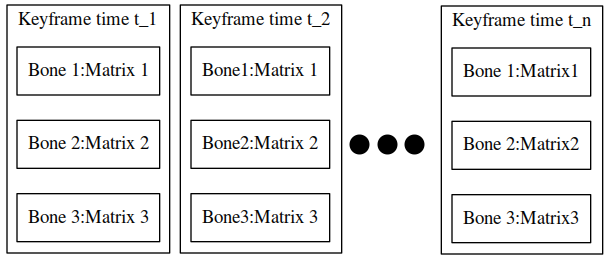
\includegraphics[width=0.4\textwidth]{anim_track.png}
    \caption{\small{В ключевые моменты времени \detokenize{(t_1, t_2, ... t_n)}, каждая кость ставиться в соответствие с матрицей локальной трансформации.}}
    
\end{figure}


\textbf{Модель}
Модель состоит из набора вершин, весов вершин (коэффициентов, определяющих влиение костей на вершину), нормалей, материалов. В пакете для трех мерной анимации модель привязывают к скелету, каждая вершина модели «привязывается» к какой-либо кости скелета (или к нескольким костям). После привязки модели к скелету при движении отдельной кости будут двигаются и все вершины, привязанные к ней.

\begin{figure}[h!]
    \centering
    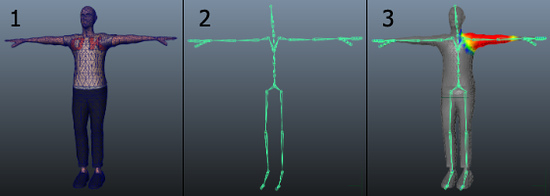
\includegraphics[width=0.6\textwidth]{skinning.png}
    \caption{\small{Слева: модель; в центре: скелет; справа: выделенны вершины модели, которые были привязанны к кости правого предплечья}}
    %\label{fig:awesome_image}
\end{figure}

%=============================================================
\subsubsection{Описание алгоритма}




Для создания эффекта анимации необходимо извлекать из трека набор матриц поворота соответствующий настоящему моменту времени. Применять этот набор матриц к скелету, а затем применять позу скелета к модели (то есть изменять координаты вершин).

\textbf{Применение данных из трека к скелету}
Матрицы поворота для всех костей записываются в треке относительно матрицы поворота родителя.
Поэтому для анимации скелета необходимо применять матрицы в последовательном порядке.
Начинаем с корневой кости и применяем к ней описанную в треке анимации матрицу поворота.
Затем, двигаемся вглубь скелета по иерархии и находим произведение матрицы родителя и матрицы потомка (извлеченной из трека). Другими словами расчитывается глобальная матрица поворота для кости-потомка.

Необходимо продолжать движение по иерархии пока не будут рассмотренны все кости. Ниже приведен псевдокод для применения данных из трека к скелету:

\begin{figure}[h!]
\begin{small}
\begin{verbatim}
deform_skeleton (bone root, matrix global, track matrices)
  get the matrix for root bone from track matrices
  multiply it by matrix global
  store the result in bone root as global transform
  if root has children
    deform (children of this node, root bone global matrix, track matrices)
  end if
end function
\end{verbatim}
\end{small}
\end{figure}

\begin{figure}[h!]
    \centering
    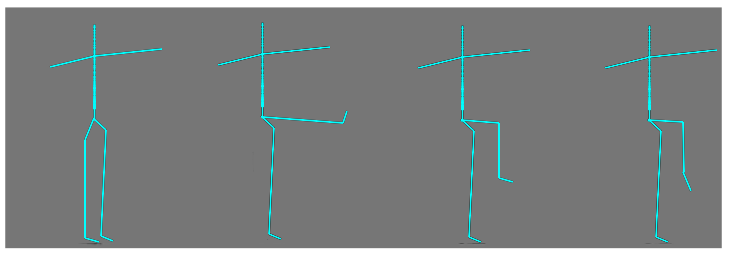
\includegraphics[width=0.6\textwidth]{forward_kinematics_skeleton.png}
    \caption{\small{Последовательное применение преобразований, начиная от копчика (корневой кости) и заканчивая ступней.}}
    %\label{fig:awesome_image}
\end{figure}


\textbf{Применение скелета к модели}

После того как рассчитанны матрицы поворотов для скелета, их необходимо применить на вершины модели.
Для этого используется рекурсивный алгоритм похожий на алгоритм для анимации скелета. Ниже приведен его псевдокод:

\begin{small}
\begin{verbatim}
deform_mesh (bone root, mesh original, mesh deformed)
  for each child_bone of root
    for each vertex in the original mesh
      if bone_weight > 0
          apply bone global transform to vertex
          scale the resulting point by the bone weight
          store the result in deformed
      end if
    end for
    if child_bone has children
      deform_mesh (children of this node, mesh original, deformed)
    end if
  end for
end function
\end{verbatim}
\end{small}

\begin{figure}[h!]
    \centering
    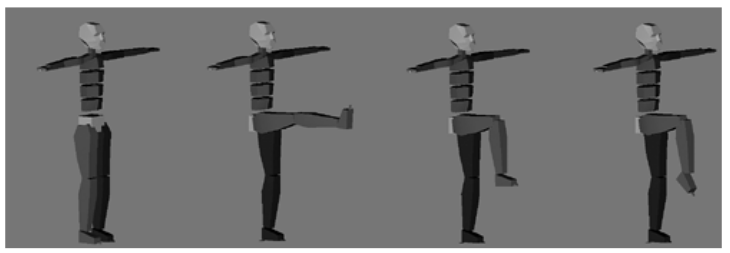
\includegraphics[width=0.8\textwidth]{forward_kinematics.png}
    \caption{\small{Применение преобразований к вершинам модели.}}

\end{figure}



\subsubsection{Реализация программы скелетной анимации}
В программе можно выделить несколько логических блоков. Каждый блок состоит из одного или более классов предоставлающих определенный функционал.

\begin{my_enumerate}
\item Блок чтения данных.
\item Блок хранения состояния анимации.
\item Блок хранения данных модели и скелета.
\item Блок деформации скелета.
\item Блок отрисовки модели.
\item Блок управления компонентами.
\end{my_enumerate}

\textbf{Чтение данных}
С помощью библиотеки Assimp производится чтение из файла. Для оптимальной работы данные перераспределяются из структур Assimp в свои. Другие функции этой библиотеки не используются.
Ниже приведен упрощенный код считывающий информацию из файла и строящий стуктуры данных.

\begin{verbatim}
// функция для загрузки данных из библиотеки Assimp, в созданные структуры данных
public void LoadScene(byte[] filedata)
{
    using (MemoryStream fs = new MemoryStream(filedata))
    {
        _cur_scene = new SceneWrapper(ReadAssimpScene(fs, "dae"));
        // во входных данных всегда только один трек анимации
        _animation_track = _cur_scene.Animations[0];
        // примененает описания из трека анимации к скелету
        _action = new Animator(_animation_track);
        // корневая кость скелета
        BoneNode bones = _cur_scene.BuildBoneNodes("Armature");
        // модель
        Node mesh = _cur_scene.FindNode("Mesh");
        // хранит состояние анимации
        ActionState state = new ActionState();
        // объединет компоненты
        _enttity = new Entity(_cur_scene, mesh, bones, state);
    }
}
\end{verbatim}


\textbf{Хранение состояния анимации}
Класс ActionState хранит состояние анимации. Наиболее важные поля:
\begin{itemize}
\item Трек анимации.
\item Настоящий момент времени в секундах.
\item Массив времени для всех ключевых кадров.
\end{itemize}

Фyнкция SetTime(\dots) используется для перехода к определенному моменту времени. Она находит интервал между ключевыми кадрами, подсчитывает величину интерполяции.

\begin{verbatim}
// функция для прыжка к определенному времени
public void SetTime(double time_seconds)
{            
    double time_ticks = time_seconds * TickPerSec;
    // когда время в секундах переполняеться, запускаем анимацию с начала
    double time = time_ticks % TotalDurationTicks;
    // поиск интервала между ключевыми кадрами
    int start_frame = FindStartFrameAtTime(time_seconds);
    int end_frame = (start_frame + 1) % KeyframeCount;
    // нахождение значения для интерполяции между ключевыми кадрами
    double delta_ticks = KeyframeTimes[end_frame] - KeyframeTimes[start_frame];
    // если необходимо запустить анимацию заново
    if (delta_ticks < 0.0)
    {
        delta_ticks += TotalDurationTicks;
    }
    double blend = (time - KeyframeTimes[start_frame]) / delta_ticks;
    // приписываем результаты расчетов
    OriginKeyframe = start_frame;
    TargetKeyframe = end_frame;
    KfBlend = blend;
}
\end{verbatim}


\textbf{Хранение данных модели и скелета}
Работает со скелетом и моделью.
Реализует функции поиска костей в скелете или подмоделей в модели.
Функция BuildBones строит скелет по данным из модели (скелет как отдельный класс не существует, он определяеться корневой костью).


\textbf{Деформация скелета}
Применяет данные, описывающие (в матрицах поворота) новую позицию для каждой кости к костям из скелета.
То есть деформирует скелет в соответствии с моментом времени в анимации. На вход блока подается класс ActionState, содержащий информацию о состоянии анимации и корневая кость скелета.

\begin{verbatim}
// функция для извлечения матриц поворота из трека и применения их к скелету
public void ChangeLocalFixedDataBlend(ActionState st)
{
    // для каждой кости создает свой канал анимации    
    foreach (NodeAnimationChannel channel in _action.NodeAnimationChannels)
    {
        BoneNode bone_nd = _scene.GetBoneNode(channel.NodeName);
        // поворот кости
        Quaternion target_roto = Quaternion.Identity;
        if (channel.RotationKeyCount > st.TargetKeyframe)
        {
            target_roto = channel.RotationKeys[st.TargetKeyframe].Value.eToOpenTK();
        }
        Quaternion start_frame_roto = channel.RotationKeys[st.OriginKeyframe].Value;
        // интерполяция поворота между двумя ключевыми кадрами
        Quaternion result_roto = Quaternion.Slerp(start_frame_roto, target_roto, (float)st.KfBlend);
        // сдвиг кости
        Vector3 target_trans = Vector3.Zero;
        if (channel.PositionKeyCount > st.TargetKeyframe)
        {
            target_trans = channel.PositionKeys[st.TargetKeyframe].Value;
        }
        Vector3 cur_trans = channel.PositionKeys[st.OriginKeyframe].Value;
        // интерполяция сдвига между двумя ключевыми кадрами
        Vector3 result_trans = cur_trans + Vector3.Multiply(target_trans - cur_trans, (float)st.KfBlend);
        // объединение поворота и сдвига
        Matrix4 result = Matrix4.CreateFromQuaternion(result_roto);
        result.Row3.Xyz = result_trans;
        bone_nd.LocalTransform = result;
    }
}

// функция для расчета глобальной матрицы поворота для каждой кости
// эта матрица будет позднее применена к вершинам модели
private void ReCalculateGlobalTransform(BoneNode nd)
{
    nd.GlobalTransform = nd.LocalTransform * nd.Parent.GlobalTransform;
    foreach (var child in nd.Children)
    {
        ReCalculateGlobalTransform(child);
    }
}
\end{verbatim}



\textbf{Отрисовка модели}
Загружает данные о модели в OpenGL.
Запрашивает OpenGL об выделение буферов памяти под вершины, нормали, цвета вершин и массив индексов. Применяет свойства материала, например: цвет, коэффициент рассеивания света, коэффициент свечения и т.д.

Данные o вершинах, материалах и нормалях необходимо загружать в буферы памяти расположенные на видеокарте для того что бы обеспечить приложению приемлимую скорость отрисовки.
Ниже приведен код для загрузки данных в память видеокарты:

\begin{verbatim}
// объект содержащий идентификационные номера буферов в OpenGL
struct Vbo
{
    public int VertexBufferId;
    public int NormalBufferId;
    public int ElementBufferId;
    public int NumIndices;
}

// функция для создания нового буфера 
// и заполнения его данными из массива векторов
private void NewOpenGLBufferWithFloats(out int outGlBufferId, List<Vector3D> dataBuffer) 
{
    GL.GenBuffers(1, out outGlBufferId);
    GL.BindBuffer(BufferTarget.ArrayBuffer, outGlBufferId);
    int sizeof_vec3d = 12; // X,Y,Z = 3 floats, 4 bytes each
    var byteCount = dataBuffer.Count * sizeof_vec3d;
    var temp = new float[byteCount];
    var n = 0;
    foreach(var v in dataBuffer)
    {
        temp[n++] = v.X;
        temp[n++] = v.Y;
        temp[n++] = v.Z;
    }
    GL.BufferData(BufferTarget.ArrayBuffer, (IntPtr)byteCount, temp, BufferUsageHint.StreamDraw);
    VerifyArrayBufferSize(byteCount);
    GL.BindBuffer(BufferTarget.ArrayBuffer, 0);
}

// функция для загрузки данных о модели в память видеокарты
private void Upload(out Vbo vboToFill)
{
    vboToFill = new Vbo();    
    NewOpenGLBufferWithFloats(out vboToFill.VertexBufferId, _mesh.Vertices);
    if (_mesh.HasNormals)
    {
        NewOpenGLBufferWithFloats(out vboToFill.NormalBufferId, _mesh.Normals);
    }
}

\end{verbatim}

Для создания эффекта движения нeобходимо каждый кадр менять содержимое буферов расположыенных на видеокарте.
А именно необходимо менять координаты вершин и направления нормалей к каждой вершине (для корректного отображения света/тени).
Для этого необходимо послать запрос к драйверу OpenGL и получить указатель на память с загруженными ранее данными.
Далее приведен код модифицирущий данные в буфере для следующего кадра.

\begin{verbatim}
// функция для получения доступа к буферу OpenGL
public void BeginModifyNormalData(out IntPtr data, out int qty_normals)
{
    GL.BindBuffer(BufferTarget.ArrayBuffer, _vbo.NormalBufferId);
    data = GL.MapBuffer(BufferTarget.ArrayBuffer, BufferAccess.ReadWrite);
    qty_normals = _mesh.Normals.Count;
}
// функция для освобождения буфера OpenGL
public void EndModifyNormalData()
{
    bool data_upload_ok = GL.UnmapBuffer(BufferTarget.ArrayBuffer);
    if (! data_upload_ok)
    {
        throw new Exception("OpenGL driver has failed.");
    }
}
\end{verbatim}


\textbf{Управление компонентами}
Класс Entity объединяет компоненты необходимые для анимации одного персонажа. Хранит ссылки на скелет (корневую кость), состояние анимации (ActionState), на саму модель и на класс отрисовки модели (MeshDraw).
    \medskip
    В частности блок персонажа применяет трансформации из скелета к вершинам модели (взвешивая действие каждой кости на вершину) и модифицирует данные в буфере данных OpenGL, что и создает эффект анимации.
    
\begin{verbatim}
// функция в блоке управления компонентами для применения матриц костей к вершинам модели
public void RecursiveTransformVertices(Node node)
{
    foreach (int mesh in nd.Meshes)
    {
        // получаем указатель на буфер в OpenGL
        IntPtr pbuf_opengl;
        int qty_vertices;
        mesh.BeginModifyVertexData(out pbuf_opengl, out qty_vertices);
        // изначальная модель без деформаций
        Mesh original_data = mesh.OriginalData;
        // go over every vertex in the mesh
        unsafe
        {
            int sz = 3;         // размер шага
            float* coords = (float*)pbuf_opengl;
            for (int vertex_id = 0; vertex_id < qty_vertices; vertex_id++)
            {
                Matrix4 matrix_with_offset = mesh._vertex_id2matrix[vertex_id];
                // получить изначальные координаты вершины
                Vector3 vertex_default = original_data.Vertices[vertex_id];
                Vector3 vertex;
                Vector3.Transform(ref vertex_default, ref matrix_with_offset, out vertex);
                // Применение веса к вершине
                Vector3 delta = vertex_default - vertex;
                vertex += delta *  mesh._vertex_id2bone_weight[vertex_id];
                // Запись новых координат обратно в буфер OpenGL
                coords[vertex_id*sz + 0] = vertex.X;
                coords[vertex_id*sz + 1] = vertex.Y;
                coords[vertex_id*sz + 2] = vertex.Z;
            }
        }
        mesh.EndModifyVertexData();

        foreach (Node child in nd.Children)
        {
            RecursiveTransformVertices(child);
        }
    }
}
\end{verbatim}


\subsection{Mетод организации входных и выходных данных}

\subsubsection{Описание метода входных и выходных данных}
Входными данными является файл в формате collada (.dae)
, в котором в обязательном порядке должны присутствовать следующие элементы:
\begin{my_enumerate}
\item Одна полигональная модель.
\item Один трек анимации.
\item Один скелет.
\end{my_enumerate}

Если не выполненны условия на наличие полигональной модели,
трека анимации и связанного с моделью скелета то
у программы не хватит информации для воспроизведения анимации.

Выходными данными является отображение анимации на экране.


\subsection{Выбор состава технических средств}

\subsubsection{Состав технических и програмных средств}
Для возможности запустить приложение необходимо учесть следующие системные требования:
\begin{my_enumerate}
\item Компьютер, оснащенный:
    \begin{my_enumerate}
    \item Обязательно 64-разрядный (x64) процессор с тактовой частотой 1 гигагерц (ГГц) или выше;
    \item 1 ГБ оперативной памяти (ОЗУ);
    \item 1.5 ГБ свободного места на жестком диске;
    \item графическое устройство OpenGL с драйвером версии 3.1 или выше.
    \end{my_enumerate}
\item Монитор
\item Видеокарта
\item Мышь
\item Клавиатура
\end{my_enumerate}
\bigskip

Также необходимо учесть следующие програмные требования:
\begin{my_enumerate}
\item Поддержка OpenGL версии 3.1
\item 64-битная операционная система Windows 7.
\item .NET Framework версии 4.5.1
\item Библиотека Assimp версии 3.1
\item Библиотека OpenTK версии 1.1.4
\end{my_enumerate}

Программа была протестирована и отлажена на версии OS Windows 7 с использованием .Net Framework 4.5.1, OpenTK версии 1.1.4 и Assimp версии 3.1.

Качество и корректность работы программы при других версиях библиотек и операционных систем не проверялось.

Программа использует буферы графической памяти типа STREAM\_WRITE и функции glMapData и glSubBufferData которые в OpenGL официально поддерживаются лишь с версии 3.1

Технические требования к памяти и периферии не превышают технических требований к операционной системе Windows 7 с установленным на ней .Net Framework 4.5.1
